\documentclass{standalone}

\begin{document}

\subsection{Aufgabe 4.3}
a) $\mathbb{L} = ]\infty, -2[ \cap ]3, \infty[$\\
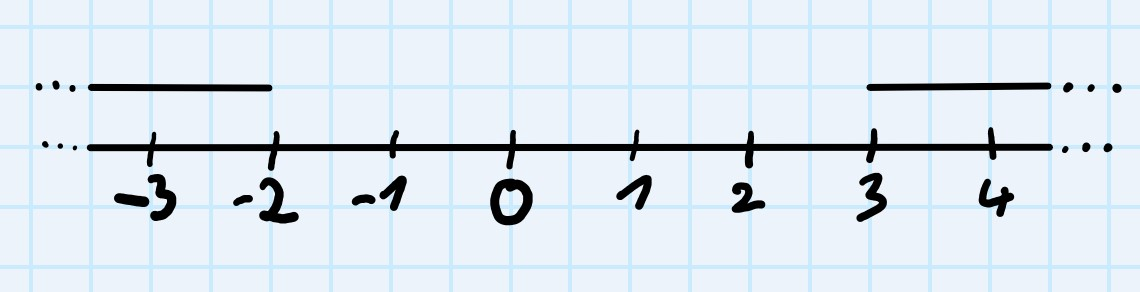
\includegraphics[scale=0.125]{4_3_a.jpg}\\ \\
b) $\mathbb{L} = [0, \infty[$\\
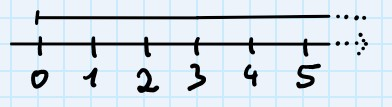
\includegraphics[scale=0.36]{4_3_b.jpg}\\ \\
c) $\mathbb{L} = \{-2, 0, 2\}$\\
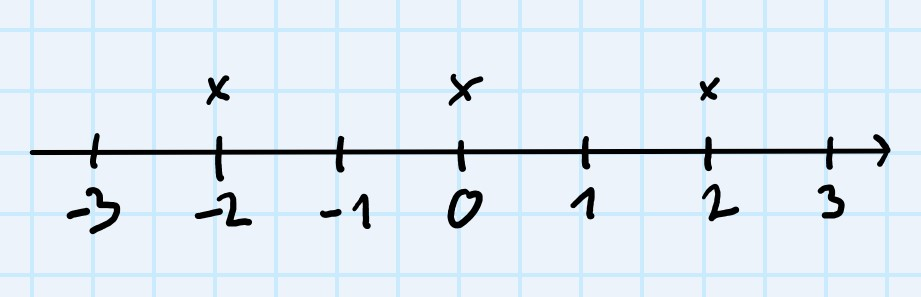
\includegraphics[scale=0.15]{4_3_c.jpg}\\

\subsection{Aufgabe 4.4}
a)\\
$2x+y<7 \rightarrow y < 7 -2x$ (grün)\\
$x-4y < 8 \rightarrow y > \frac{x}{4} - 2$ (blau)\\
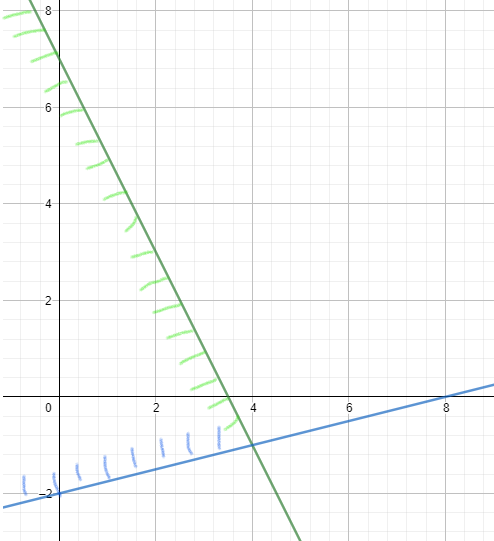
\includegraphics[scale= 0.5]{4_4_a.png}\\
Die Lösungsmenge ist der schraffierte Raum.
\newpage

\noindent b)\\
$ y \leq 3x-1$ (grün)\\
$ y \leq \frac{x}{2} + 4$ (blau)\\
$ y = -x + 7$ (rot)\\
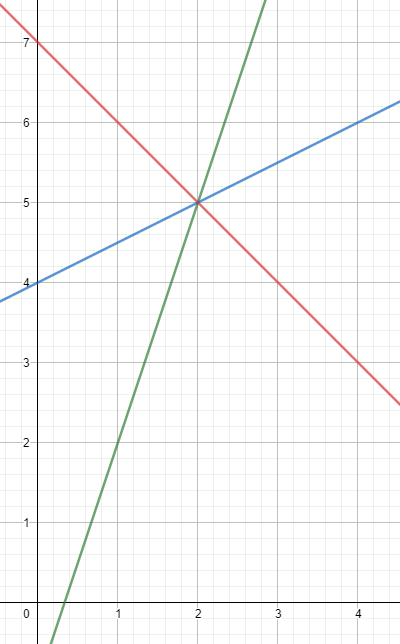
\includegraphics[scale= 0.5]{4_4_b.png}\\
$\mathbb{L} =\{(2, 5)^T\}$\\

\end{document}
